\documentclass{proc}

\usepackage{amsmath}
\usepackage{amsthm}
\usepackage{amssymb}
\usepackage{amsbsy}
\usepackage{graphicx}
\usepackage[outdir=./]{epstopdf}
\usepackage[round]{natbib} 
\usepackage{url}
\usepackage{subcaption}
\usepackage{hyperref}
\usepackage{hyphenat}
\usepackage{pdfpages}
\usepackage{MnSymbol} %udots
\usepackage{afterpage} %\afterpage{\clearpage}
\usepackage{siunitx} %for measurements

\setcounter{tocdepth}{2}
\setcounter{secnumdepth}{2}

\let\footruleskip\undefined
\usepackage{fancyhdr}
\pagestyle{plain}

\DeclareMathOperator{\variance}{\mathbb{V}ar}
\DeclareMathOperator{\normal}{N}
\DeclareMathOperator*{\argmax}{argmax}

\newcommand{\addNumber}[1]{\protect\input{#1}\unskip}
\newcommand{\inputNumber}[1]{\protect\input{#1}\unskip}

\title{Local normalisation using the empirical null for inspection of additive manufacturing using a single x-ray projection}
\date{2019}
\author{
  Sherman Lo \and Gregory Gibbons \and Thomas Nichols \and Julia Brettschneider \and Mark Williams \and Jason Warnett
}

\begin{document}\sloppy

\maketitle

\begin{abstract}
X-ray computed tomography can be used for defect detection in additive manufacturing. Typically, x-ray projections of an object are taken at a number of angles that are then reconstructed to create a 3D representation of the object inclusive of internal features. To avoid this time consuming process, it was investigated whenever it is possible to detect defects based on a single angular projection. A 3D printed sample was manufactured with voids to see if they can be detected. The x-ray acquisition was compared with a simulation of that scan under the face of uncertainty by treating each pixel as a hypothesis test. The empirical null filter locally normalises each test statistic using robust estimators of the mean and deviation so that sensible inference was achieved. Voids with diameters in the order of millimetres were detectable.
\end{abstract}

\section{Introduction}

Quality control in additive manufacturing can be done using x-ray computed tomography (CT) \citep{thompson2016x}. The CT is compared with the computer aided design (CAD) so that voids and surface deviation can be measured in terms of position and size \citep{villarraga2015assessing, lee2015compliance, kim2016inspection}. The disadvantage of x-ray CT is that it involves the acquisition and reconstruction of thousands of projections of the sample. Speeding up the quality control process on the production line could be done by doing an inspection using a fewer number of projections by sacrificing accuracy \citep{warnett2016towards, brierley2018optimized}.

A method was proposed to compare a single projection with a simulation of that projection and treating it as the ground truth. This was done by using two-tailed multiple hypothesis testing \citep{pearson1900on, neyman1933on, fisher1970statistical} controlling the false discovery rate (FDR) \citep{benjamini1995controlling, benjamini2010discovering}, treating each pixel as an individual test. Beforehand however, the empirical null \citep{efron2004large} was used to do local normalisation on the test statistics. This was necessary because the simulation of the projection did not perfectly reproduce the obtained projection, leading to incorrect inference.

An x-ray projection of a 3D printed sample was obtained and compared with the simulation in an experiment. The procedure is shown in the methods section along with the description of the empirical null filter. In addition, the software development and simulation studies of the filter was discussed. The results from the simulation and the experiment are shown in the results section. The conclusion section summarises the study along with a discussion on further work.

\section{Methods}

\subsection{Apparatus and Data Collection}

An ABS plastic cuboid (\SI{40}{\milli\metre} $\times$ \SI{40}{\milli\metre} $\times$ \SI{60}{\milli\metre}) with voids was purposefully manufactured to see if they can be detected. The CAD shown in Figure \ref{fig:inference_testObject} was manufactured using a \emph{Fortus 400mc (Stratasys, US)} 3D printer. The voids were of diameters \SI{2.4}{\milli\metre}, \SI{1.2}{\milli\metre}, \SI{0.6}{\milli\metre} and \SI{0.3}{\milli\metre}. 6 voids for each diameter were designed in the CAD. Voids with diameters \SI{2.4}{\milli\metre} and \SI{0.6}{\milli\metre} were regularly arranged, otherwise they were arranged irregularly. The precision of the manufacturing was in the order of $\pm\SI{0.1}{\milli\metre}$.

\begin{figure}
  \centering
  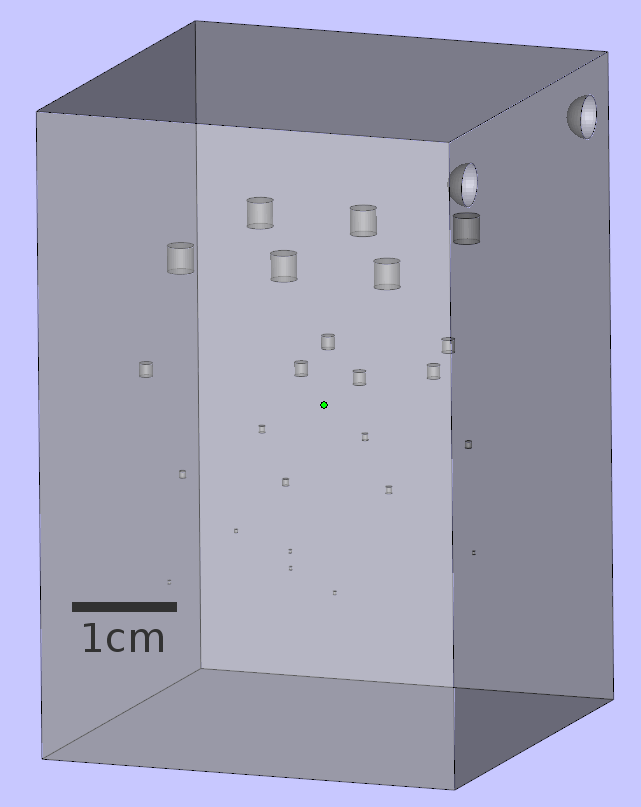
\includegraphics[width=0.35\textwidth]{../figures/inference/TestObject.png}
  \caption{CAD of a 3D cuboid with voids. The voids were of diameters \SI{2.4}{\milli\metre}, \SI{1.2}{\milli\metre}, \SI{0.6}{\milli\metre} and \SI{0.3}{\milli\metre}. 6 voids for each diameter were designed in the CAD. Voids with diameters \SI{2.4}{\milli\metre} and \SI{0.6}{\milli\metre} were regularly arranged, otherwise they were arranged irregularly. The scale shown is approximate.}
  \label{fig:inference_testObject}
\end{figure}

X-ray projections were obtained using the \emph{Nikon XT H LC 225/320} x-ray CT scanner \emph{(Nikon Metrology, UK)}. The \SI{225}{\kilo\volt} source was used with a $2000\times2000$ pixel \emph{Perkin Elmer} detector consisting of \SI{200}{\micro\metre} pixels, separated by a distance of \SI{1870}{\milli\metre}. The sample was placed on the manipulator, positioned to obtain a $5.7\times$ magnification resulting in an equivalent pixel size of \SI{35}{\micro\metre}. A voltage of \SI{80}{\kilo\volt} was used with a power of \SI{20}{\watt} resulting in a spot size of \SI{20}{\micro\metre} such that penumbra effects were negligible. 20 greyscale projections were acquired at an exposure time of \SI{500}{\milli\second}. A shading correction \citep{young2000shading, munzenmayer2003enhancing} was applied to each projection using a black (\SI{0}{\kilo\volt}) and white image (\SI{80}{\kilo\volt}) projection to remove intensity influences and variations in pixels of the detector.

The projection of the 3D printed sample was obtained and repeated 20 times at a fixed angle. The 20 projections were spilt into 2. 19 random projections were held out. The remaining projection was used to compare with the simulation using \emph{aRTist} \citep{bellon2007artist, jaenisch2008artist, bellon2012radiographic}. In the \emph{aRTist} simulation, the software did a simulation as if the voids were not there. Numerical methods were used to align the simulated projection to the obtained projection.

\subsection{Statistical Methodology}

Two-tailed multiple hypothesis testing \citep{pearson1900on, neyman1933on, fisher1970statistical} was used to quantify the disagreement of each pixel between the projection and the \emph{aRTist} projection. A disagreement too big will classify that pixel as a positive result. A test statistic $Z_{x,y}$ for the $(x,y)$ positioned pixel was calculated for all pixels. This test statistic, together makes a $z$ image, is
\begin{equation}
  Z_{x,y} = 
  \dfrac{
    \text{projection}_{x,y} - \emph{aRTist}_{x,y}
  }
  {
    \sqrt{\widehat{\variance}\left[\text{projection}_{x,y}\right]}
  }
\end{equation}
where $\widehat{\variance}\left[\text{projection}_{x,y}\right]$ is the estimated grey value variance of pixel $(x,y)$ in the projection.

The variance model, $\widehat{\variance}\left[\text{projection}_{x,y}\right]$ has a linear relationship between the variance and the grey value \citep{yang2010noise}. The fitting of the model was done using the held out replicated projections of the sample. These replicated projections were manually segmented. This provided variance-mean data, where each pixel is a data point, and was used to fit the variance model. The model used was a gamma distributed generalised linear model \citep{nelder1972generalized, mccullagh1984generalized} with an identity link. The variance was predicted using the grey value in the \emph{aRTist} projection as the predictor variable when working out the test statistics.

It was assumed that the grey values were Normal, therefore the test statistics should be approximately Normal as well. Let the test statistic of the pixel at position $(x,y)$ be
\begin{equation}
Z_{x,y}\sim\normal(\mu_{x,y},\widehat{\sigma}_{0,x,y}^2)
\end{equation}
for $x=1,2,\cdots,W$ and $y=1,2,\cdots,H$. $\mu_{0,x,y}$ and $\sigma_{0,x,y}$ are the null mean and null standard deviation at position $(x,y)$ respectively. Their estimates are $\widehat{\mu}_{0,x,y}$ and $\widehat{\sigma}_{0,x,y}$ also respectively. Define the null hypotheses to be
\begin{equation}
  H_{0,x,y}:\mu_{x,y}=\widehat{\mu}_{0,x,y}
\end{equation}
which are tested against
\begin{equation}
  H_{1,x,y}:\mu_{x,y}\neq\widehat{\mu}_{0,x,y} \ .
\end{equation}
The empirical null filter aims to obtain the estimators $\widehat{\mu}
_{0,x,y}$ and $\widehat{\sigma}_{0,x,y}$ for all $x$ and $y$. This is based on the empirical null \citep{efron2004large} where hypothesis testing is done by comparing a test statistic with the empirical distribution of the majority of the test statistics rather than a specified null distribution.

To obtain the estimates, a circular kernel with radius $r$ was centred at $(x,y)$. All the pixels captured by the circular kernel and the region of interest (ROI) were pooled together to obtain a kernel density estimate \citep{parzen1962on, friedman2001elements}
\begin{equation}
\widehat{p}_{Z_{x,y}}(z) = 
\frac{1}{nh}
  \sum_{i,j\in K_{x,y}}\phi\left(
    \dfrac{z_{i,j}-z}{h}
  \right)
\end{equation}
where $K_{x,y} = \text{kernel centred at }(x,y) \cap \text{ROI}$, $n$ is the number of pixels captured by $K_{x,y}$, $\phi(z)$ is the probability density function of a standard Normal random variable and $h$ is the bandwidth. The bandwidth was chosen such that
\begin{equation}
  h = (0.9n^{-1/5}\ + 0.16) \times \text{min}\left(s_{x,y},\text{IQR}_{x,y}/1.34\right)
  \label{eq:inference_ourruleofthumb}
\end{equation}
where $s_{x,y}$ and $\text{IQR}_{x,y}$ are the sample standard deviation and sample interquartile range of the test statistics in $K_{x,y}$, similar to \cite{silverman1986density, sheather2004density}. The estimates were obtained by solving
\begin{equation}
\widehat\mu_{0,x,y} = \text{argmax} \widehat{p}_{Z_{x,y}}(z)
\end{equation}
using the Newton-Raphson method and
\begin{equation}
  \widehat{\sigma}_{0,x,y} = \left[
    \left.
      -\dfrac{\partial^2}{\partial z^2}\ln\widehat{p}_{Z_{x,y}}(z)
    \right|_{z=\widehat{\mu}_{0,x,y}}
  \right]^{-1/2}
\end{equation}
\citep{efron2004large}. The test statistics were normalised using
\begin{equation}
  T_{x,y} = 
  \dfrac{
    Z_{x,y}-\widehat{\mu}_{0,x,y}
  }
  {
    \widehat{\sigma}_{0,x,y}
  } \ .
\end{equation}
All the normalised test statistics were converted to $p$-values
\begin{equation}
  p_{x,y} = 2(1-\Phi(|t_{x,y}|))
\end{equation}
and was used in the \cite{benjamini1995controlling} (BH) procedure at the 5\% FDR level to classify pixels as positive or not for defects.

\subsection{Software Development}

The empirical null filter was implemented using \emph{ImageJ} \citep{abramoff2004image, schindelin2012fiji, schneider2012nih, perez2013image} by modifying the existing class \texttt{RankFilters}. It contains implementations of filters, such as the mean filter and median filter, using a circular kernel and multiple threads. Each thread filters a row in parallel.

Line filtering was done from left to right. At the start on the far left, an initial value of the median of all the test statistics in the kernel was used. For the following pixel to the right, the empirical null mean of the neighbouring left pixel was used as the initial point. This was chosen as it was assumed the empirical null mean would vary slowly and smoothly spatially.

When filtering a pixel, the Newton-Raphson method was used to solve for $\widehat{\mu}_{0,x,y}=z$
\begin{equation}
  \dfrac{\partial}{\partial z}\ln\widehat{p}_{Z_{x,y}}(z) = 0
\end{equation}
by using the iterative procedure
\begin{equation}
  z^{(r+1)} =
  z^{(r)}
  -\dfrac{
    \left.
      \dfrac{
        \partial
      }
      {
        \partial z
      }
      \ln\widehat{p}_{Z_{x,y}}(z)
    \right|_{z = z^{(r)}}
  }
  {
    \left.
      \dfrac{
        \partial^2
      }
      {
        \partial z^2
      }
      \ln\widehat{p}_{Z_{x,y}}(z)
    \right|_{z = z^{(r)}}
  } 
\end{equation}
where $z^{(0)}$ is the initial value. A convergence criteria was met when either 10 update steps were taken or when
\begin{equation}
  \log\left[\left|
    \left.
    \dfrac{
      \partial
    }
    {
      \partial z
    }
  \ln\widehat{p}_{x,y}(z)
  \right|_{z=z^{(r)}}
  \right|\right]
  <-5
\end{equation}
at the current step. This was chosen arbitrary to speed up the algorithm without losing too much accuracy. The solution is valid if
\begin{equation}
  \left.
    \dfrac{
      \partial^2
    }
    {
      \partial z^2
    }
    \ln\widehat{p}_{Z_{x,y}}(z)
  \right|_{z=\widehat{\mu}_{0,x,y}}
  < 0 \ .
\end{equation}
Further initial values were generated by sampling from $\normal(z^{(0)}, s_{x,y}^2)$. This was done multiple times until 3 valid solutions were obtained. The best solution, the one with the largest $\ln\widehat{p}_{Z_{x,y}}\left(\widehat{\mu}_{0,x,y}\right)$, out of all the different initial values was used as the final answer.

\subsection{Simulation}

The empirical null filter was tested to see if it can detect simulated defects from a $\SI{256}{px}\times \SI{256}{px}$ contaminated image. A defect is a pixel which has a value not distributed under the null distribution, but instead an alternative distribution. For example suppose $Z_{x,y}|H_{0,x,y}\sim\normal(0,1)$, then a defect would have a value distributed as $Z_{x,y}|H_{1,x,y}\sim\normal(\mu_{1},1)$ where $\mu_1\neq0$. A $\SI{30}{px}\times \SI{30}{px}$ square defect was simulated. A kernel can capture the entire defect if its radius is large enough.

Contamination is the result of a linear transform of the test statistics $Z_{x,y}$. For example in this experiment, the image was multiplied by 2 and a gradient was added to it. Suppose the image does contain defects, then an example of a resulting distribution is
\begin{align}
  Z_{x,y}|H_{0,x,y}&\sim\normal(\mu_{0,x,y},2^2)
  \\
  Z_{x,y}|H_{1,x,y}&\sim\normal(2\mu_1+\mu_{0,x,y},2^2)
\end{align}
where $\mu_{0,x,y}=0.01(x-x_0)+0.01(y-y_0)$ and $(x_0,y_0)$ is the centre of the image. This was used in this study to simulate a contaminated image with defects. The contaminated square defected image is shown in Figure \ref{fig:inference_defectSquare2Example}.

\begin{figure}
  \centering
  \includegraphics[width=0.4\textwidth]{../figures/inference/defectSquare2Example_imageContaminated.eps}
  \caption{A $\SI{256}{px}\times \SI{256}{px}$ contaminated Gaussian image with a $\SI{30}{px} \times \SI{30}{px}$ square defect. The null and alternative distributions are $Z_{x,y}|H_{0,x,y}\sim\normal(\mu_{0,x,y},2^2)$ and $Z_{x,y}|H_{1,x,y}\sim\normal(6+\mu_{0,x,y},2^2)$ respectively where $\mu_{0,x,y}=0.01(x-x_0)+0.01(y-y_0)$ and $(x_0,y_0)$ is the centre of the image.}
  \label{fig:inference_defectSquare2Example}
\end{figure}

The contamination is a nuisance because the test statistics will have larger variance and larger values at the two corners. This will cause an inflation in false positives which will lead to incorrect inference. 

Literature, such as \cite{efron2004large} and \cite{schwartzman2008empirical}, suggest that, as a rule of thumb, the proportion of non-null statistics should not be larger than $0.1$ to satisfy some assumptions made for the empirical null. In this simulated example, it is about $r>\SI{54}{px}$. A kernel too small would treat the defects as null, making them difficult to detect.

The receiver operating characteristic (ROC) curve \citep{green1966signal, metz1978basic, hanley1982meaning, friedman2001elements, cook2007use} was studied in this experiment. The ROC is a parametric plot, plotting the true positive rate (sensitivity) against the false positive rate ($1-\text{specificity}$) for varying thresholds. The area under the ROC curve is a commonly used statistic to quantify the performance of the test \citep{friedman2001elements}. Interpretations of the area do exist \citep{metz1978basic,hanley1982meaning} and discussed thoroughly in \cite{cook2007use}.

A simulation study was conducted where the contaminated defected image was filtered for various kernel radiuses for $\mu_1=3$. Hypothesis testing was done on the uncontaminated defected image and filtered contaminated defected image. The area under the ROC curve and various errors were recorded. This was repeated 100 times by simulating another image. To form a baseline to compare with, the results of the uncontaminated image were all pooled together to obtain the empirical distribution of the ROC area and errors without contamination.

\begin{figure*}[p]
  \centering
    \centerline{
      \begin{subfigure}{0.49\textwidth}
        \includegraphics[width=\textwidth]{../figures/inference/DefectRadiusSquare_roc.eps}
        \caption{ROC area}
      \end{subfigure}
      \begin{subfigure}{0.49\textwidth}
        \includegraphics[width=\textwidth]{../figures/inference/DefectRadiusSquare_type1.eps}
        \caption{Type 1 error}
      \end{subfigure}
    }
    \centerline{
      \begin{subfigure}{0.49\textwidth}
        \includegraphics[width=\textwidth]{../figures/inference/DefectRadiusSquare_type2.eps}
        \caption{Type 2 error}
      \end{subfigure}
      \begin{subfigure}{0.49\textwidth}
        \includegraphics[width=\textwidth]{../figures/inference/DefectRadiusSquare_fdr.eps}
        \caption{FDR}
      \end{subfigure}
    }
  \caption{ROC area and various errors obtained when conducting a hypothesis test on a $\SI{256}{px} \times \SI{256}{px}$ filtered contaminated Gaussian image with a $\SI{30}{px}\times \SI{30}{px}$ square defect. Various kernel radiuses were investigated. The dashed lines show the resulting 95\% empirical confidence interval when the hypothesis test was done on the uncontaminated image with a defect. The null and alternative distributions are $Z_{x,y}|H_{0,x,y}\sim\normal(\mu_{0,x,y},2^2)$ and $Z_{x,y}|H_{1,x,y}\sim\normal(6+\mu_{0,x,y},2^2)$ respectively where $\mu_{0,x,y}=0.01(x-x_0)+0.01(y-y_0)$ and $(x_0,y_0)$ is the centre of the image. The test was done at the 5\% FDR level. The box plot summarise the 100 repeated measurements of the experiment.}
  \label{fig:inference_Experiment_DefectRadiusSquare}
\end{figure*}

\section{Results}

The result from the simulation is shown Figure \ref{fig:inference_Experiment_DefectRadiusSquare}. The ROC area increased with kernel radius which highlighted that a filtered image with a good radius kernel can performance almost as well as though there was no contamination. It also appeared that the optimal ROC area was achieved when using the kernel radius from the rule of thumb, making these results consistent with literature.

Keeping the FDR consistent before and after filtering is desirable so that the FDR is kept controlled at a specified level after filtering. For large enough kernel radius, the FDR was controlled at around, perhaps a bit below, 5\%. It appeared a large kernel radius helped preserve FDR control after filtering in these examples. 

It appeared there is a kernel radius which minimised the type 2 error. A large kernel radius is required for FDR control but too large can lose statistical power.

In the experiment with the 3D printed sample, the x-ray projection was manually segmented further as shown in Figure \ref{fig:inference_segmentFurther}. It was segmented using the edges of the projection of the 3D printed sample. The empirical null filter was then used on each segment, or ROI, independently, ignoring any pixels outside the ROI the filter is working on. The resulting filtered segments were stitched together to form the resulting filtered image. The resulting inference is shown in Figure \ref{fig:inference_subroiAbsFilterDeg120_inference_radius4}.

The larger defects were successfully highlighted by the hypothesis test. It can be seen that the empirical null mean did change face to face, resulting in a clear boundary set by the edges. This probably suggest that the contamination or inaccuracy from \emph{aRTist} was face dependent.

\begin{figure}
  \centering
  \includegraphics[width=0.45\textwidth]{../figures/inference/segment.JPG}
  \caption{The x-ray projection was segmented further into 7 segments or ROI.}
  \label{fig:inference_segmentFurther}
\end{figure}

\begin{figure*}
  \centering
    \centerline{
      \begin{subfigure}[b]{0.49\textwidth}
        \includegraphics[width=\textwidth]{../figures/inference/DefectDetectSubRoiAbsFilterDeg120_radius4_sig.eps}
        \caption{X-ray projection with positive pixels}
      \end{subfigure}
      \begin{subfigure}[b]{0.49\textwidth}
        \includegraphics[width=\textwidth]{../figures/inference/DefectDetectSubRoiAbsFilterDeg120_radius4_logp.eps}
        \caption{$-\log p$}
      \end{subfigure}
    }
    \centerline{
      \begin{subfigure}{0.49\textwidth}
        \includegraphics[width=\textwidth]{../figures/inference/DefectDetectSubRoiAbsFilterDeg120_radius4_nullMean.eps}
        \caption{Empirical null mean}
      \end{subfigure}
      \begin{subfigure}{0.49\textwidth}
        \includegraphics[width=\textwidth]{../figures/inference/DefectDetectSubRoiAbsFilterDeg120_radius4_nullStd.eps}
        \caption{Empirical null std}
      \end{subfigure}
    }
  \caption{Resulting inference when using the empirical null filter, on each segment independently, with radius $r=\SI{130}{px}$. a) X-ray projection with highlighted red positive pixels at the 5\% FDR level. b) $p$-values on the log scale. c) and d) Empirical null mean and standard deviation.}
  \label{fig:inference_subroiAbsFilterDeg120_inference_radius4}
\end{figure*}

\section{Conclusion}

The empirical null filter caters for inaccuracies made by \emph{aRTist} and voids in the order of millimetres were detectable. This demonstrated that the filter can adjust the null hypotheses according to the data to make sensible inference. In the experiments, it was found that the FDR level is preserved after filtering.

False positives do occur but this is unavoidable because tests were done at the 5\% FDR level. Typically in the experiments, false positives were isolated single pixels and probably occurred due to random chance. Clusters of positive pixels should raise suspicion. One could create a binary image, assigning a Boolean value whether that pixel was tested positive or not. A binary image filter, such as erode followed by a dilate, can be used to remove isolated positive pixels to emphasise the cluster of positive pixels.

For good results, the faces of the 3D printed cuboid were segmented. This was necessary because the empirical null filter assumes that the null parameters varied spatially smoothly and slowly. Manual segmentation was easy to do because a cuboid has 6 faces. However, segmentation of faces cannot be generalised well to 3D printed samples with complicated geometry and curved surfaces.

The main issue was how slow the filter was. Figure \ref{fig:inference_timing} shows the timings of the empirical null filter and the mean variance filter. For a filter to take more than a minute is unacceptable when used on the production line when typical filters can take a fraction of a second.

\begin{figure*}
  \centering
    \centerline{
      \begin{subfigure}[b]{0.49\textwidth}
        \includegraphics[width=\textwidth]{../figures/inference/AllNullGaussianEmpirical_time.eps}
        \caption{Empirical null filter}
      \end{subfigure}
      \begin{subfigure}[b]{0.49\textwidth}
        \includegraphics[width=\textwidth]{../figures/inference/AllNullGaussianMeanVar_time.eps}
        \caption{Mean variance null filter}
      \end{subfigure}
    }
  \caption{Timings when filtering a $\SI{256}{px}\times \SI{256}{px}$ image. The mean variance null filter uses the sample mean and sample standard deviation to locally normalise the image. Note that the $y$-axis changes scale. The box plot summarise 100 repeated measurements of the timings.}
  \label{fig:inference_timing}
\end{figure*}

There are a few strategies to accelerate the filter. The empirical null filter may be accelerated using GPUs \citep{yang2008parallel, hwu2011gpu, eklund2013medical}, however efforts to implement the filter in \emph{CUDA} and \emph{C++} is fruitless if there may exist a faster method. Instead, accuracy may be sacrificed for speed by only estimating the null parameters for a number of regularly spaced pixels, the remaining pixels then do estimation through interpolation. The problem is that the assumption of a slow varying null parameter is required much more because of the use of interpolation, this may cause bigger problems due to the face to face transition observed in the experiments. It was found that if a bad solution was found for a point, then that solution would spread its bad solution to neighbour pixels due to the interpolation.

The main bottleneck is the evaluation of the density estimate, each step in the Newton-Raphson required the evaluation of each pixel in the kernel. Perhaps there may be faster methods for density estimation such as fitting a smoothing spline on the histogram \citep{efron2004large}, however that would require tuning the histogram bins as well as the tuning parameters for the spline. On the other hand, the method in \cite{schwartzman2008empirical} which uses the histogram count found that the estimation of the null parameters was insensitive to the histogram binning.

Estimation of the null parameters is essentially robust statistics, estimating the parameters of the null distribution without being affected by non-null statistics. Potential faster methods than the empirical null could exist in literature for robust statistics such as \cite{hampel1986robust, rousseeuw1987robust, maronna2006robust, huber2009robust, jewson2018principles}. The EM algorithm \citep{dempster1977maximum} could be used to fit a mixture of Gaussians to identify the null distribution and estimate its parameters. However the power of hypothesis testing and the empirical null comes from the fact that the alternative distribution does not need to be specified.

\section{Acknowledgements}
This work is funded by EPSRC grant numbers EP/K031066/1 (Inside-out: Statistical methods for Computed Tomography validation of complex structures in Additive Layer Manufacturing) and EP/L016710/1 (EPSRC and MRC Centre for Doctoral Training in Next Generation Statistical Science: The Oxford-Warwick Statistics Programme).

\bibliographystyle{apalike}
\bibliography{../bib}

\end{document}
